\documentclass[12pt]{article}

\input{/home/iasbeck/preamble.tex}

\lhead{} % Lado esquerdo do cabeçalho
\chead{} % Centro do cabeçalho
\rhead{} % Lado direito  do cabeçalho
\lfoot{} % Lado esquerdo do rodapé
\cfoot{} % Centro do rodapé
\rfoot{\thepage} % Lado direito  do rodapé

% Folha A4
% Margem superior = Margem esquerda = 3cm
% Margem direita = Margem inferior = 2cm
% Fonte Times New Roman 12
% Títulos de Figuras e Tabelas Times New Roman 10
% Espaçamento simples e alinhamento justificado

% Início do documento
\begin{document}
	\singlespacing % Espaçamento simples
	%\pagestyle{empty} % Remove numeração das páginas
	
	% Inserção da capa
	\thispagestyle{empty}
	\newgeometry{top=1.5cm, bottom=2cm, left=2cm, right=2cm} 
	
	\begin{figure}[H]
		\centering
		
\includegraphics[width=\linewidth]{cabecalho.png}
	\end{figure}
	
	\begin{center}
		\large
		\textbf{UNIVERSIDADE FEDERAL DE UBERLÂNDIA} \\ \vspace{0.3cm}
		\textbf{FACULDADE DE ENGENHARIA MECÂNICA} \\~\\~\\~\\~\\~\\~\\~\\
		\Large
		\textbf{LISTA DE OTIMIZAÇÃO CLÁSSICA} \\~\\~\\~\\~\\~\\~\\
		\large
		\textbf{ARTHUR HENRIQUE IASBECK} \\~\\~\\~\\~\\~\\~\\~\\
		\large
		\textbf{UBERLÂNDIA} \\
		\textbf{17 DE OUTUBRO DE 2019}
	\end{center}
	\newpage
	\restoregeometry
	
	\setcounter{page}{1} % Impede que a capa seja contada na paginação
	
	% ==============================================================================================
	% EXERCÍCIO 1 ==================================================================================
	% ==============================================================================================
	
	\section*{EXERCÍCIO 1}
		No Exercício 1 foi proposto um problema baseado no posicionamento de carros interconectados por molas, que tinha como objetivo a minimização da energia potencial associada ao sistema. A função a ser minimizada neste caso é apresentada na Eq. \ref{fOjb1}
		\begin{equation}
			f(X) = \frac{1}{2}X^TKX - X^TP
			\label{fOjb1}
		\end{equation}
		
		\noindent sendo
		\begin{gather}
			X = \left[ \begin{array}{ccc} x_1 & x_2 & x_3 \end{array} \right]^T \\
			P = \left[ \begin{array}{ccc} 1000 & 2000 & 3000 \end{array} \right]^T \\
			K = \left[ \begin{array}{ccc} 8500 & -1000 & -2500 \\ -1000 & 3000 & -500 \\ -2500 & -500 & 11500 \end{array} \right]
		\end{gather}                                  
		
		Efetuando a multiplicação matricial introduzida na Eq. \ref{fOjb1} obtém-se $ f(x) $, Eq. \ref{fx}.
		\begin{equation}
			\begin{split}
				f(x) = 4250x_1^2 - 1000 x_1 x_2 - 2500 x_1 x_3 - 1000 x_1 + 1500 x_2^2 \\
				- 500 x_2 x_3 - 2000 x_2 + 5750 x_3^2 - 3000 x_3 \label{fx}
			\end{split}
		\end{equation}
		
		A partir da relação introduzida na Eq. \ref{fx} é possível determinar analiticamente $ \nabla f(x) $, Eq \ref{gradF}.
		\begin{equation}
			\nabla f(x) = \left[ \begin{array}{ccc}
			8500 x_1 - 1000 x_2 - 2500 x_3 - 1000 \\
			3000 x_2 - 1000 x_1 -500 x_3 - 2000 \\
			11500 x_3 - 500 x_2 - 2500 x_1 - 3000
			\end{array} \right]
			\label{gradF}
		\end{equation} 
		
		O Método das Variáveis Métricas foi empregado para determinação de $ x^* $. Esta abordagem é baseada no Método de Newton e propõe uma aproximação para a inversa da Matriz Hessiana, que deve ser atualizada recursivamente. Assim sendo, a cada iteração $ x^{k+1} $ é determinado a partir das Eqs. \ref{atualizaX} e \ref{s}. 
		\begin{gather}
			x^{k+1} = x^k + \alpha s^k \label{atualizaX} \\
			s^k = - \nabla f(x^k)H^k \label{s}
		\end{gather}
		
		
		\noindent sendo $ H $ uma aproximação para a inversa da Matriz Hessiana. É necessário que a mesma seja atualizada ao fim de cada iteração por meio do emprego das Eqs. \ref{atualizaH} a \ref{atualizaD}.
		\begin{gather}
			H^k = H^{k-1} + D^{k-1} \label{atualizaH} \\
			p = x^k - x^{k-1} \\
			y = \nabla f(x^k) - \nabla f(x^{k-1}) \\
			\sigma = p^T y \\
			\tau = y^T H^k y \\
			D^k = \frac{\sigma + \theta \tau}{\sigma^2} pp^T + \frac{\theta - 1}{\tau} (H^k y)(H^k y)^T - \frac{\theta}{\sigma} (H^k y p^T + p(H^k y)^T) \label{atualizaD}
		\end{gather}
		
		Pode-se adotar $ \theta = 1 $ ou $ \theta = 0 $. No presente trabalho ambas as possibilidades foram consideradas. 
		
		É importante ressaltar que neste caso é necessário que a ordem do problema seja reduzida, de forma a torná-lo uni-dimensional, para que seja possível determinar o valor ótimo de $ \alpha $, que será utilizado na determinação de $ x^{k+1} $, Eq. \ref{atualizaX}. Essa redução se dá em todas as iterações e para operá-la adotou-se
		\begin{equation}
			g(\alpha) = f(x^{k-1} - \alpha H \nabla f(x^{k-1})) \label{reducao}
		\end{equation} 
		
		Observe que a relação introduzida na Eq. \ref{reducao} foi baseada naquela apresentada na Eq. \ref{atualizaX} e que $ x^{k-1} $, $ H $ e $ \nabla f(x) $ são conhecidos, de forma que a única variável que resta é o próprio $ \alpha $. Uma vez minimizada $ g(\alpha) $ é determinado $ \alpha^* $ e já é possível empregar a Eq. \ref{atualizaX} para determinação de $ x^{k+1} $. 
		
		O código no qual foi implementado o Método das Variáveis métricas é apresentado a seguir. Para minimização de $ g(\alpha) $ e determinação de $ \alpha^* $ foi empregado o Método da Seção Áurea, que foi implementado de forma genérica em \mcode{[xOpt, fOpt, k] = aureaSec(f,a,b,tol)}, sendo \mcode{xOpt} o ponto de ótimo determinado pelo processo de otimização, \mcode{f} a função a ser minimizada, \mcode{fOpt} o valor de $ f(x^*) $, \mcode{k} o numero de chamadas de $ f(x) $, \mcode{a} e \mcode{b} os extremos do espaço de busca, e \mcode{t} a tolerância adotada para encerramento das iterações.
		
		\begin{lstlisting}
clc; clear; close all;

addpath('..');

% Parametros pra execucao do algoritmo
n = 3;
numGrad = 0; 
x0 = [0, 0, 0]';
tol = 1e-4;

% Definicao da funcao objetivo
f = @(x) 4250*x(1).^2 - 1000*x(1)*x(2) - 2500*x(1)*x(3) - 1000*x(1) + ...
1500*x(2).^2 - 500*x(2)*x(3) - 2000*x(2) + 5750*x(3).^2 - 3000*x(3);

if numGrad
	% Definicao numerica do gradiente
	h = 1e-10;
	df = @(x) [(f([x(1) + h, x(2), x(3)]) - f([x(1), x(2), x(3)]))/h
	(f([x(1), x(2) + h, x(3)]) - f([x(1), x(2), x(3)]))/h
	(f([x(1), x(2), x(3) + h]) - f([x(1), x(2), x(3)]))/h];
else 
	% Definicao analitica do gradiente
	df = @(x) [8500*x(1) - 1000*x(2) - 2500*x(3) - 1000
	3000*x(2) - 1000*x(1) - 500*x(3) - 2000
	11500*x(3) - 500*x(2) - 2500*x(1) - 3000];
end

% Variaveis para controle de execucao
alfaOptValues = zeros(1,1);
k = 1;
nVal = 0;
H = eye(n);

while 1 
	% Reduzir a dimensao do problema de otimizacao
	g = @(alfa) f(x0 - alfa*H*df(x0));
	
	% Resolver o problema de otimizacao uni-dimensional
	[alfaOpt,~,nVal1] = aureaSec(g,-1,1,1e-4);
	
	% Atualizar a solucao otima
	x = x0 - alfaOpt*H*df(x0);
	
	% Armazenar dados de execucao 
	alfaOptValues(k) = alfaOpt;
	if numGrad 
		nVal = nVal + nVal1 + 6;
	else
		nVal = nVal + nVal1 + 1; 
	end
	
	% OBS : Lembre-se que e necessaria a computacao do gradiente para atualizacao de x. No entanto, se estivermos utilizando a aproximacao numerica para o gradiente, a computacao do mesmo levara, neste caso a 6 avaliacoes da funcao objetivo.
	
	% Verificar a condicao de parada
	cp = norm(x - x0);
	if cp < tol
		break;
	end
	
	% Atualizacao de H (aproximacao para a inversa da Matriz Hessiana)
	p = x - x0;
	y = df(x) - df(x0);
	sigma = p'*y;
	tal = y'*H*y;
	theta = 1;
	D = ((sigma + theta*tal)/sigma^2)*(p*p') ...
	+ ((theta - 1)/tal)*(H*y)*(H*y)' ...
	- (theta/sigma)*(H*y*p' + p*(H*y)');
	
	H = H + D;
	
	% Atualizar variaveis para a proxima iteracao
	x0 = x;
	k = k + 1;
end

xOpt = x;
fOpt = f(xOpt);

for i = 1:length(x)
	fprintf(['x',num2str(i),'* = %.4f\n'], xOpt(i));
end

fprintf('f(x*) = %.4f\n', fOpt);
fprintf('Numero de avaliacoes da funcao objetivo: %d\n', nVal);
fprintf('Numero de iteracoes: %d\n', k);
		\end{lstlisting} 
	
	\vspace{0.4cm}
	É importante ressaltar que a forma como o Método da Variável Métrica foi implementado possibilita que seja empregado tanto o gradiente calculado analiticamente quanto aquele obtido numericamente, bastando que seja modificada a variável \mcode{numGrad}.
	
	Os resultados obtidos a partir da execução do algoritmo apresentado são introduzidos na Tab. \ref{resultados}. É interessante observar que, para o estudo de caso em questão, a forma como é computado o gradiente não influencia no valor de $ x^* $, assim como o valor de $ \theta $ também não foi relevante na solução do problema de otimização. Cabe ressaltar, no entanto, que a computação numérica do gradiente leva a um maior número de avaliações da função objetivo. 
	
	\begin{table}[H]
		\centering
		\caption{Resultados obtidos a partir da implementação do Método da Variável Métrica.}
		\label{resultados}
		\begin{tabular}{|c|c|c|c|c|c|c|c|}
			\hline
			\begin{tabular}[c]{@{}c@{}}Computação do\\ gradiente\end{tabular} & $\theta$ & $x_1^*$                 & $x_2^*$                & $x_3^*$                 & $f(x^*)$                    & $n_{val}$            & $k$                \\ \hline
			\multirow{2}{*}{Numérica}                                         &     0            & \multirow{4}{*}{0,3241} & \multirow{4}{*}{0,836} & \multirow{4}{*}{0,3677} & \multirow{4}{*}{-1549,5888} & \multirow{2}{*}{140} & \multirow{4}{*}{5} \\ \cline{2-2}
			& 1        &                         &                        &                         &                             &                      &                    \\ \cline{1-2} \cline{7-7}
			\multirow{2}{*}{Analítica}                                        & 0        &                         &                        &                         &                             & \multirow{2}{*}{115} &                    \\ \cline{2-2}
			& 1        &                         &                        &                         &                             &                      &                    \\ \hline
		\end{tabular}
	\end{table}

	A implementação do Método da Seção Áurea pode ser avaliado abaixo. 
	\begin{lstlisting}
function [xOpt, fOpt, k] = aureaSec(f,a,b,tol)
	tal = 0.618;
	
	if nargin < 4
	tol = 1e-8;
	end
	
	alfa = a + (1 - tal)*(b - a);
	beta = a + tal*(b - a);
	fAlfa = f(alfa);
	fBeta = f(beta);
	
	k = 1;
	
	while abs(a-b) > tol
		if fBeta < fAlfa 
			a = alfa;
			alfa = beta;
			fAlfa = fBeta;
			beta = a + tal*(b - a);
			fBeta = f(beta);
		elseif fAlfa <= fBeta
			b = beta;
			beta = alfa;
			fBeta = fAlfa;
			alfa = a + (1 - tal)*(b - a);
			fAlfa = f(alfa);
		end
		k = k + 1;
	end
	
	xOpt = (alfa+beta)/2;
	fOpt = f(xOpt);
	
end
	\end{lstlisting}
	
	Todos os códigos introduzidos nos presente trabalho podem ser acessados no link \url{https://github.com/ArthurIasbeck/OTMC3}.
	
	% ==============================================================================================
	% EXERCÍCIO 2 ==================================================================================
	% ==============================================================================================
	
	\section*{EXERCÍCIO 2}
	
	No Exercício 2 foi proposta a solução de Problemas de Programação Linear a partir do emprego do Método Gráfico. As funções a serem minimizadas ou maximizadas, denotadas por $ f_1(x) $, $ f_2(x) $ e $ f_3(x) $ são introduzidas nas Eqs. \ref{f1}, \ref{f2} e \ref{f3}. 
	\begin{gather}
		min \; f_1(x) = 2 x_1 \label{f1} \\
		max \; f_2(x) = -4 x_2 \label{f2} \\
		max \; f_3(x) = 3 x_1 + 3  \label{f3} 
	\end{gather} 
	
	As restrições às quais estão sujeitas $ f_1(x) $, $ f_2(x) $ e $ f_3(x) $ são apresentadas nas Eqs. \ref{rest1} a \ref{rest5}.
	\begin{gather}
		-x_1 + 2 x_2 \leq 0 \label{rest1} \\
		2 x_1 - 3 x_2 \leq 3 \label{rest2} \\
		x_1 + 3 x_2 \leq 6 \label{rest3} \\
		x_1 \geq 0 \label{rest4} \\
		x_2 \geq 0 \label{rest5} 
	\end{gather} 
	
	A implementação do Método Gráfico para minimização ou maximização de $ f_1(x) $, $ f_2(x) $ e $ f_3(x) $ pode ser verificada nas Figs. \ref{f1Img}, \ref{f2Img} e \ref{f3Img}.
	
	\begin{figure}[H]
		\centering
		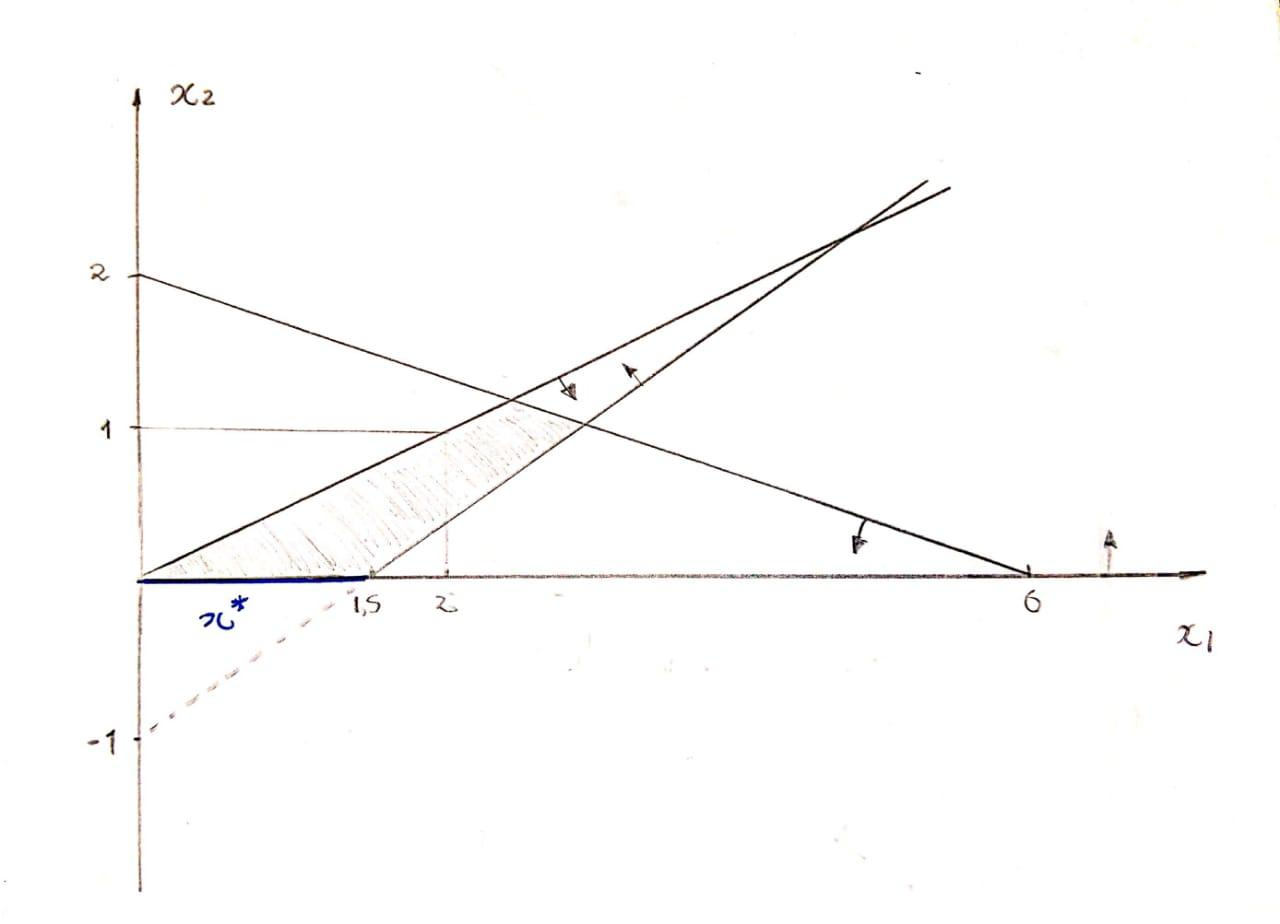
\includegraphics[width=0.8\linewidth]{figuras/1.jpeg}
		\caption{Resultado da implementação do método gráfico para minimização de $ f_1(x) $. }
		\label{f1Img}
	\end{figure}

	\begin{figure}[H]
		\centering
		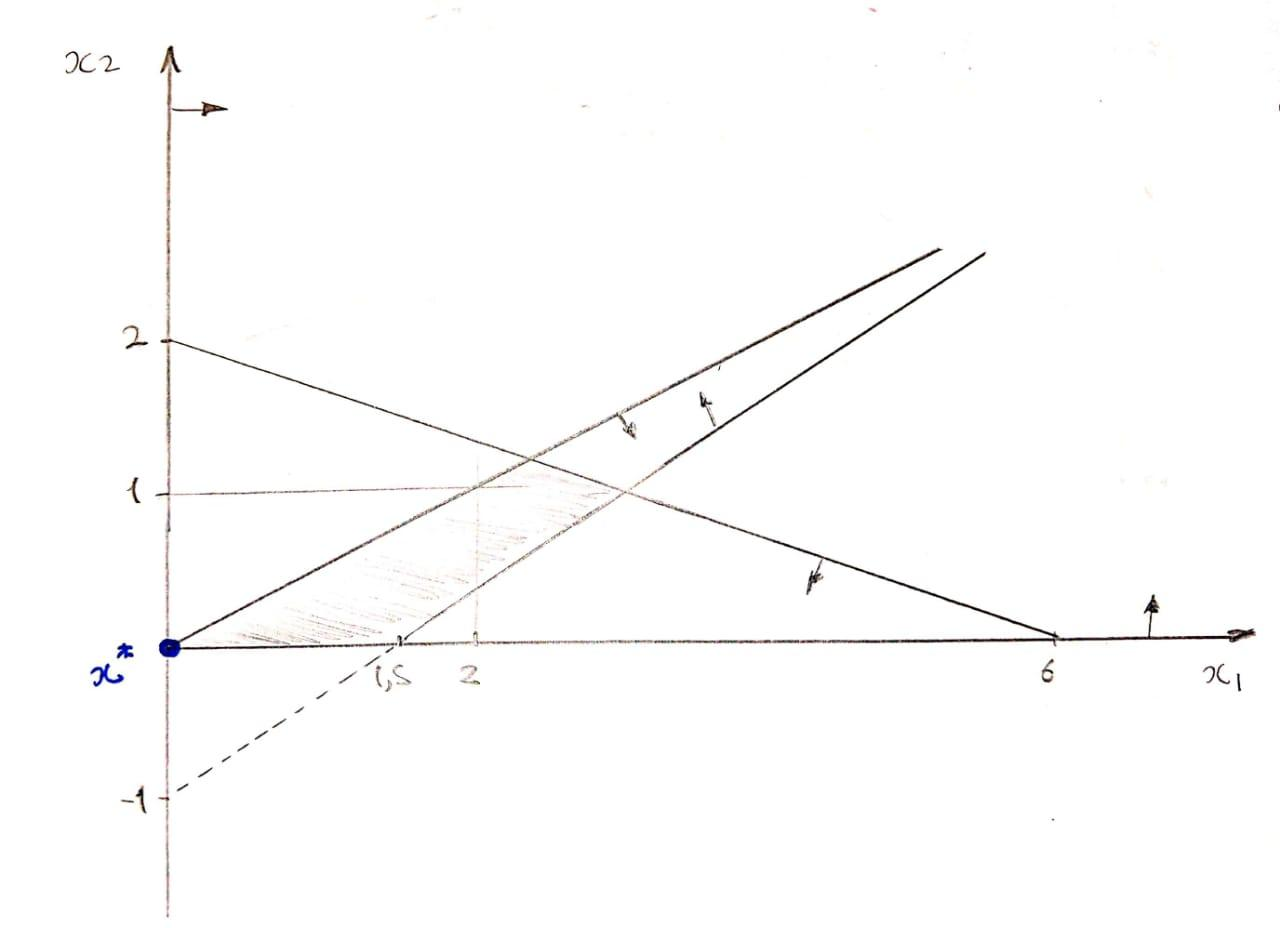
\includegraphics[width=0.8\linewidth]{figuras/2.jpeg}
		\caption{Resultado da implementação do método gráfico para minimização de $ f_2(x) $. }
		\label{f2Img}
	\end{figure}

	\begin{figure}[H]
		\centering
		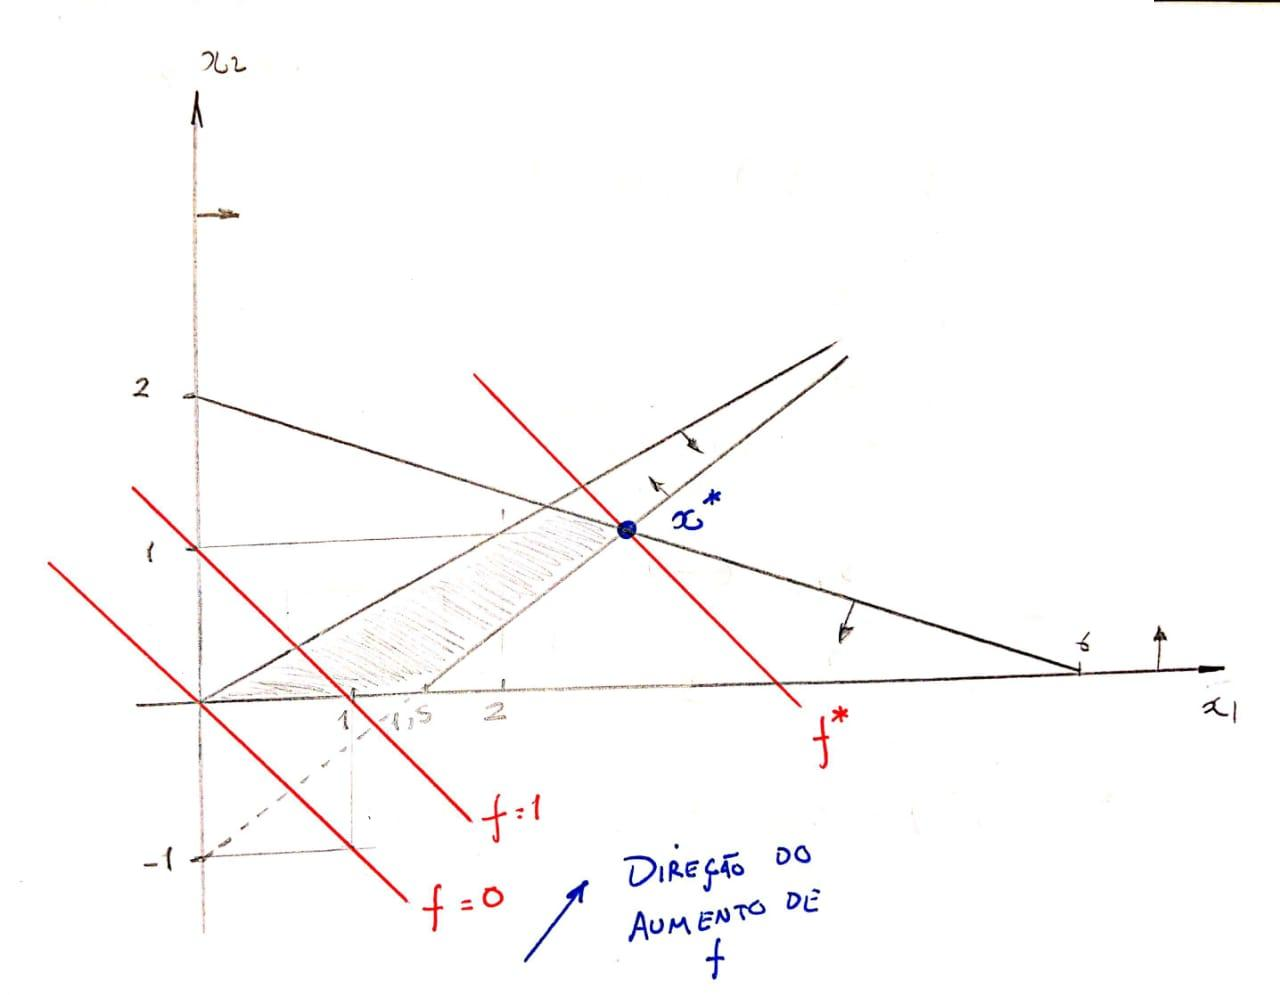
\includegraphics[width=0.8\linewidth]{figuras/3.jpeg}
		\caption{Resultado da implementação do método gráfico para minimização de $ f_3(x) $. }
		\label{f3Img}
	\end{figure}
	
	É possível observar que a partir da minimização de $ f_1(x) $ são obtidas infinitas soluções para $ x^* $, uma vez que o valor de $ f_1(x) $ depende somente de $ x_1 $, que deve ser igual a zero para que $ f_1(x) $ seja minimizado. Já a maximização de $ f_2(x) $ conduz a $ x^* = \left[ \begin{array}{c c} 0 & 0 \end{array} \right] $. A maximização de $ f_3(x) $ por sua vez, indica que $ x^* $ se encontra na interseção das retas construídas a partir das restrições introduzidas nas Eqs. \ref{rest2} e \ref{rest3}, o que implica que a determinação de $ x^* $ se dá pela solução do sistema 
	\begin{eqnarray}
		\begin{cases}
			2 x_1^* - 3 x_2^* = 3 \\
			x_1^* + 3 x_2^* = 6
		\end{cases}
	\end{eqnarray}
 	
 	\noindent de forma que $ x_1^* = 3 $ e $ x_2^* = 1 $.
 	
 	% ==============================================================================================
 	% EXERCÍCIO 3 ==================================================================================
 	% ==============================================================================================
 	
 	\section{EXERCÍCIO 3}
 	
 	No Exercício 3 foi proposta a solução do Problema de Programação Linear descrito em Carpio, R. C; Silva, R. J.; Jorge, A. B. \textit{“Otimização da Mistura de Combustíveis Secundários Alternativos Visando Atender as Restrições Operacionais e Ambientais em Fornos de Cimenteiras”}. Foi proposta neste caso a função objetivo introduzida na Eq. \ref{fObj3}.
 	\begin{equation}
	 	\begin{split}
		 	min \; f(x) = 0,93 x_1 + 0,54 x_2 + 1,54 x_3 + 0,77 x_4 + 35 x_5 + 40 x_6 - 50 x_7 \\
		 	 + 0,031((5,76ms - 5,82) e^{-0,2ms + 0,98})
		 	\label{fObj3}
	 	\end{split}
 	\end{equation}
 	
 	\noindent sendo 
 	\begin{equation}
	 	ms = \frac{5 x_1 + 61,62 x_2 + 93 x_3 + 7,6 x_4 + 9,32 x_5 + 22 x_7}{1,86 x_1 + 25,6 x_2 + 4,07 x_3 + 84,1 x_4 + 12,29 x_5 + 10,54 x_7}
 	\end{equation}
 	
 	Além disso, o estudo de caso proposto apresenta 19 restrições de ordem operacional, representadas como restrições de igualdade e desigualdade, todas elas lineares. 
 	
 	Para verificação da influência da parcela não linear de $ f(x) $ na determinação da solução do problema, foram adotadas duas abordagens. Na primeira delas, esta parcela não linear foi desconsideradas e $ x^* $ foi determinado a partir do emprego de uma rotina do Matlab\textsuperscript{\textregistered} chamada \mcode{linprog}. Já na segunda abordagem, a parcela não linear de $ f(x) $ foi levada em consideração e a obtenção de $ x^* $ se deu a partir da implementação de outra rotina do Matlab\textsuperscript{\textregistered} denominada \mcode{fmincon}. Cabe ressaltar que ambas as funções recebem como entrada restrições de desigualdade do tipo $ Ax \leq b $, o que implica que restrições da forma $ Ax \geq b $ devem ser transformadas multiplicando-se ambos os lados por $ -1 $.
 	
 	Os resultados obtidos em cada uma das abordagens são apresentados na Tab. \ref{resultados3}. O valor de $ f(x^*) $ apresentado por Carpio \textit{et al.} foi o mesmo obtido no emprego da primeira abordagem. Além disso, como era esperado, a consideração da parcela não linear acabou por acarretar um aumento no valor da função objetivo, apesar de terem sido observadas mudanças pouco significativas no valor de $ x^* $.
 	
 	% Please add the following required packages to your document preamble:
 	% \usepackage{multirow}
 	\begin{table}[H]
 		\centering
 		\caption{Resultados obtidos a partir da minimização de $ f(x) $, ora levando em conta sua parcela não linear e ora desconsiderando-a.}
 		\label{resultados3}
 		\begin{tabular}{|c|c|c|}
 			\hline
 			\multirow{2}{*}{} & \multicolumn{2}{c|}{Abordagem} \\ \cline{2-3} 
 			& 1              & 2             \\ \hline
 			$x_1$             & 1,21928        & 1,21938       \\ \hline
 			$x_2$             & 0,22635        & 0,21749       \\ \hline
 			$x_3$             & 0              & 0             \\ \hline
 			$x_4$             & 0              & 0,00842       \\ \hline
 			$x_5$             & 0              & 0             \\ \hline
 			$x_6$             & 0,07841        & 0,07841       \\ \hline
 			$x_7$             & 0,02804        & 0,02804       \\ \hline
 			$f$               & 2,991          & 3,376         \\ \hline
 		\end{tabular}
 	\end{table}
 
 	Os códigos empregados na implementação das abordagens 1 e 2, respectivamente, são apresentados a seguir.
 	
 	\begin{lstlisting}	
clc; clear; close all; format long;

% As restricoes sao representadas matricialmente, logo, cada linha da
% matriz A representa uma retricao de desigualdade, enquanto cada linha da
% matriz Aeq representa uma restricao de igualdade. 

% Restricoes de desigualdade
A = [-50.6 -1.23 -1.13 -0.71 -1.03 0 -0.93 
     50.6 1.23 1.13 0.71 1.03 0 0.93
     -5.04  -61.62  -93  -7.6 -9.32 0 -1.93
     5.04 61.62 93 7.6 9.32 0 1.93 
     -1.19 -16.59 -2.87 -1.13 -5.08 0 -0.09
     1.19 16.59 2.87 1.13 5.08 0 0.09
     -0.67 -9.01 -1.2 -82.97 -7.21 0 -0.13 
     0.67 9.01 1.2 82.97 7.21 0 0.13
     0.78 0 0.1 0 0.44 0 0.12 
     -0.762 -2.74 -83.64 185.83 18.96 0 -1.422
     0.018 -7.5 82.011 -219.47 -23.88 0 1.335
     -0.319 -4.877 -1.31 106.73 4.29 0 0.074
     -0.619 -7.737 -0.37 -222.88 -14.387 0 -0.25
     -38.24 155.67 173.6 164.34 37.86 0 2.93
     35.48 -190.65 -212.43 -201 -46.51 0 -3.78
     0 0 0 0 0.046 0.07 0.0123
     0 0 0 0 25392 34436 0];

b = [-62 67 -9 25 -2 9 -1 5 6.5 0 0 0 0 0 0 0.05 2700];

% Restricoes de igualdade
Aeq = [0 0 0 0 25392 34436 32100
0 0 0 0 0 0 32100];
beq = [3600 900];

% Restricoes laterais
lb = [0 0 0 0 0 0 0];

f = [0.93 0.54 1.54 0.77 35 40 -50];

x = linprog(f,A,b,Aeq,beq,lb);

C = f*x;

display(x);
display(C);
 	\end{lstlisting}
 	
 	\begin{lstlisting}
clc; clear; close all; format long; 

fun = @fObj;
x0 = rand(1,7);
% Restricoes de desigualdade
% Restricoes de desigualdade
A = [-50.6 -1.23 -1.13 -0.71 -1.03 0 -0.93 
     50.6 1.23 1.13 0.71 1.03 0 0.93
     -5.04  -61.62  -93  -7.6 -9.32 0 -1.93
     5.04 61.62 93 7.6 9.32 0 1.93 
     -1.19 -16.59 -2.87 -1.13 -5.08 0 -0.09
     1.19 16.59 2.87 1.13 5.08 0 0.09
     -0.67 -9.01 -1.2 -82.97 -7.21 0 -0.13 
     0.67 9.01 1.2 82.97 7.21 0 0.13
     0.78 0 0.1 0 0.44 0 0.12 
     -0.762 -2.74 -83.64 185.83 18.96 0 -1.422
     0.018 -7.5 82.011 -219.47 -23.88 0 1.335
     -0.319 -4.877 -1.31 106.73 4.29 0 0.074
     -0.619 -7.737 -0.37 -222.88 -14.387 0 -0.25
     -38.24 155.67 173.6 164.34 37.86 0 2.93
     35.48 -190.65 -212.43 -201 -46.51 0 -3.78
     0 0 0 0 0.046 0.07 0.0123
     0 0 0 0 25392 34436 0];

b = [-62 67 -9 25 -2 9 -1 5 6.5 0 0 0 0 0 0 0.05 2700];

% Restricoes de igualdade
Aeq = [0 0 0 0 25392 34436 32100
0 0 0 0 0 0 32100];
beq = [3600 900];

% Restricoes laterais
lb = [0 0 0 0 0 0 0];

x = fmincon(fun,x0,A,b,Aeq,beq,lb);

C = fun(x);

display(x);
display(C);

function F = fObj(x)
	ms = (5*x(1) + 61.62*x(2) + 93*x(3) + 7.6*x(4) + 9.32*x(5) + 22*x(7))/ ...
	(1.86*x(1) + 25.6*x(2) + 4.07*x(3) + 84.1*x(4) + 12.29*x(5) + ...
	10.54*x(7));
	F = 0.93*x(1) + 0.54*x(2) + 1.54*x(3) + 0.77*x(4) + 35*x(5) + ...
	40*x(6) - 50*x(7) + 0.031*((5.76*ms - 5.82)*exp(-0.2*ms + 0.98));
end
 	\end{lstlisting}
 
\end{document}